\chapter{Neural Networks}
Artificial neural networks are computing systems inspired by the biological neural networks that constitute animal brains. An ANN is based on a collection of connected units or nodes called \textbf{artificial neurons}, which loosely model the neurons in a biological brain. Each connection, like the synapses in a biological brain, can transmit a signal to other neurons. An artificial neuron receives a signal then processes it and can signal neurons connected to it. The signal at a connection is a real number, and the output of each neuron is computed by some non-linear function of the sum of its inputs. The connections are called \textbf{edges}. Neurons and edges typically have a \textbf{weight} that adjusts as learning proceeds. The weight increases or decreases the strength of the signal at a connection. Neurons may have a threshold such that a signal is sent only if the aggregate signal crosses that threshold. Typically, neurons are aggregated into layers. Different layers may perform different transformations on their inputs. Signals travel from the first layer, to the last layer, possibly after traversing the layers multiple times.

\begin{wrapfigure}{l}{0.35\textwidth}
    \begin{center}
        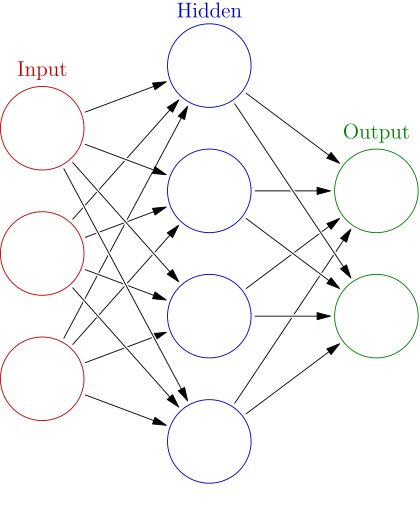
\includegraphics[width=0.25\textwidth]{053}
        \caption{An artificial neural network as an interconnected group of nodes.}
    \end{center}
    \label{fig:053}
\end{wrapfigure}

The idea of neural networks began unsurprisingly as a model of how neurons in the brain function, termed 'connectionism' and used connected circuits to simulate intelligent behaviour .In 1943, portrayed with a simple electrical circuit by neurophysiologist Warren McCulloch and mathematician Walter Pitts. Donald Hebb took the idea further in his book, The Organization of Behaviour (1949), proposing that neural pathways strengthen over each successive use, especially between neurons that tend to fire at the same time thus beginning the long journey towards quantifying the complex processes of the brain.

Around this time, Frank Rosenblatt, a psychologist at Cornell, was working on understanding the comparatively simpler decision systems present in the eye of a fly, which underlie and determine its flee response. In an attempt to understand and quantify this process, he proposed the idea of a Perceptron in 1958, calling it \textbf{Mark I Perceptron}. It was a system with a simple input output relationship, modeled on a McCulloch-Pitts neuron, proposed in 1943 by Warren S. McCulloch, a neuroscientist, and Walter Pitts, a logician to explain the complex decision processes in a brain using a linear threshold gate. A McCulloch-Pitts neuron takes in inputs, takes a weighted sum and returns '0' if the result is below threshold and '1' otherwise.

\begin{figure}[h]
    \centering
    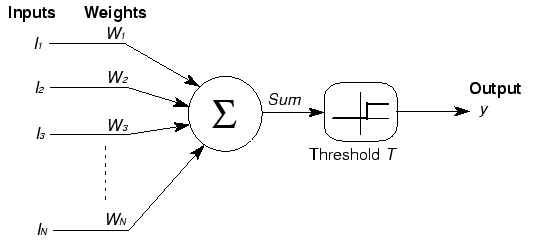
\includegraphics[width=.75\textwidth]{048}
    \caption{A McCulloch-Pitts neuron.}
\end{figure}

A major drawback? This perceptron could only learn to separate linearly separable classes, making the simple but non-linear exclusive-or circuit an insurmountable barrier.

\section{From Perceptron to Deep Networks}
In 1969 it was formally proved that perceptron cannot be used for non-linearly separable problems. In particular, it has been proved that the \textbf{XOR} (exclusive or) cannot be solved with the perceptron. We can realize the XOR as a function that map all pairs of input \(x_1\) and \(x_2\) to an output \(y\) with the following scheme:
\begin{table}[h!]
\begin{center}
\begin{tabular}{|p{0.8cm}|p{1.2cm}|p{1.2cm}|}
    \hline
    \(x_1\) & \(x_2\) & \(y\) \\
    \hline
    1 & 1 & 0 \\
    \hline
    1 & 0 & 1 \\
    \hline
    0 & 1 & 1 \\
    \hline
    0 & 0 & 0 \\
    \hline
\end{tabular}
\end{center}
\caption{XOR truth table}
\end{table} 

Despite the messy and somewhat dis-satisfactory advent of the use of Machine Learning to quantify decision systems apart from the brain, today's artificial neural networks are nothing more than \textbf{several layers of these perceptrons}.

\subsubsection{Multi-Layer Perceptron}
The idea of the multi-layer perceptron is to densely connect artifical neurons to realize compositions of non-linear functions. THe information is propagated from the inputs to the outputs. No cycles between outputs and inputs (DAG). Compute one or more non-linear function. Computation is carried out by composition of some number of algebraic functions implemented by the connections, weights and biases of the hidden and output layers. Hidden layers compute intermediate representations.

One of the problems that arose was with the impractically long runtimes required for running these networks given that this was the 60s apart from its inability to learn simple boolean exclusive-or circuits.

Multi-layer networks use a variety of learning techniques, the most popular being backpropagation. Here, the output values are compared with the correct answer to compute the value of some predefined error-function. By various techniques, the error is then fed back through the network. Using this information, the algorithm adjusts the weights of each connection in order to reduce the value of the error function by some small amount. After repeating this process for a sufficiently large number of training cycles, the network will usually converge to some state where the error of the calculations is small. In this case, one would say that the network has learned a certain target function.

\subsection{Backpropagation}
\textbf{Backpropagation}, a method devised by researchers since the 60's and continuously developed on well into the AI winter, was an intuition based method that attributed reducing significance to each event as one went farther back in the chain of events. Backpropagation along with Gradient Descent forms the backbone and powerhouse of neural networks. While Gradient Descent constantly updates and moves the weights and bias towards the minimum of the cost function, backpropagation evaluates the gradient of the cost w.r.t. weights and biases, the magnitude and direction of which is used by gradient descent to evaluate the size and direction of the corrections to weights and bias parameters.

\begin{figure}[h!]
    \centering
    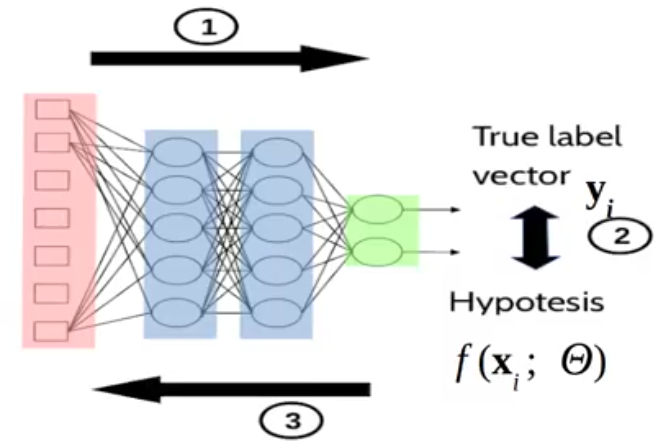
\includegraphics[width=.5\textwidth]{050}
    \caption{Backpropagation scheme.}
\end{figure}

\subsubsection{In a nutshell}
\begin{enumerate}
    \item Forward propagation: sum inputs, produce activations, feed-forward.
    \item Error estimation.
    \item Back propagate the error signal and use it to update weights.
\end{enumerate}
The main idea is that given training samples \(T = \{(x_1, y_1), (x_2, y_2), ..., (x_n, y_n)\}\), adjust the weights of the network \(\Theta\) such that a cost function is minimized
\begin{equation}
    \min_{\Theta} \sum_i L(y_i, f(x_i; \Theta))
\end{equation}
Choose the loss function (e.g. L2), update the weights of each layer with gradient descend, and use backpropagation of the error signal to compute the gradient efficiently.

\section{Feedforward Networks}
A feedforward neural network is an artificial netowkr wherein connections between the nodes do not form a cycle. The feedforward neural network was the first and simplest type of artificial neural network devised. In this network, the information moves in only one direction --- forward --- from the input nodes, through the hidden nodes (if any) and to the output nodes.

Feedforward neural networks are the quintessential deep learning models. The goal of a feedforward network is to approximate some function \(f^*: \mathcal{X} \to \mathcal{Y}\). For example, for a classifier, \(y = f^*(\vec{x})\) maps an input \(\vec{x}\) to a category \(y\). A feedforward network defines a mapping \(\vec{y} = f(\vec{x}; \vec{\Theta})\) and learns the value of the parameters \(\vec{\Theta}\) that result in the best function approximation.

Feedforward neural networks are called \textbf{networks} because they are typically represented by composing together many different functions. The model is associated with a directed acyclic graph describing how the functions are composed together. For example, we might have three functions \(f^{(1)}\), \(f^{(2)}\), and \(f^{(3)}\) connected in a chain, to form \(f(\vec{x}) = f^{(3)}(f^{(2)}(f^{(1)}(\vec{x})))\). 

\begin{figure}[h]
    \centering
    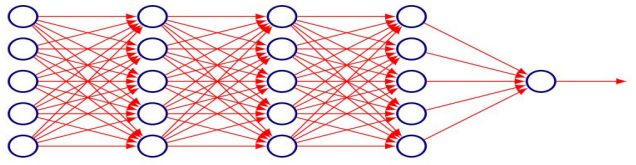
\includegraphics[width=.75\textwidth]{049}
    \caption{The function \(f\) is a composition of multiple functions.}
\end{figure}

These chain structures are the most commonly used structures of neural networks. In this case, \(f^{(1)}\) is called \textbf{first layer} of the network, \(f^{(2)}\) is the \textbf{second layer} of the network, and so on. The overall length of the chain gives the \textbf{depth} of the model. The final layer is the \textbf{output layer} of the model.

\subsection{Training}
During the training, we drive \(f(\vec{x}; \Theta)\) to match \(f^*(\vec{x})\). The training data provides us with noisy, approximate examples of \(f^*(\vec{x})\) evaluated at different training points.

The training examples specify directly what the output layer must do at each point \(\vec{x}\); it must produce a value that is close to \(y\). The behavior of the other layers is not directly specified by the training data. The learning algorithm must decide how to use those layers to produce the desired output, but the training data do not say what each individual layer should do. Instead, the learning algorithms must decide how to use these layers to best implement an approximation of \(f^*\). Because the training data does not show the desired output for each of these layers, they are called \textbf{hidden layers}.

Designing and training a neural network is not much different from training any other machine learning model with gradient descent. The largest difference between the linear models we have seen so far and neural networks is that the nonlinearity of a neural network causes most interesting loss functions to become non-convex. This means that neural networks are usually trained by using iterative, gradient-based optimizers that merely drive the cost function to a very low value, rather than the linear equation solvers used to train linear regression models or the convex optimization algorithms with global convergence guarantees used to train logistic regression or SVMs. Convex optimization converges starting from any initial parameters.

\begin{figure}[t!]
    \centering
    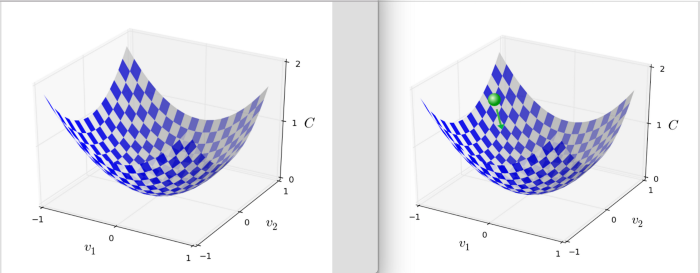
\includegraphics[width=.75\textwidth]{054}
    \caption{Ball diagram depicting the visualization of how gradient based learning occur.}
\end{figure}

In order to apply gradient descent to train our neural network, we need to specify our model, that means that we need to specify the input and output layers are made, and also the cost function.

\subsubsection{Cost Function}
The cost function, for any other machine learning algorithm, is the loss function that measures the discrepancy between the prediction of the model given the current parameters and the ground truth labels.

It is common for neural network, when we have classification problems, to apply cost function that is called \textbf{cross-entropy loss}. It is common for neural networks to transform the outputs (scores/logits) to probability, then we can think that a good cost function can be this:
\begin{equation}
    \mathcal{L}_i = - \sum_k y_k \log(S(l_k)) = -log(S(l))
\end{equation}
That is the cross-entropy loss. The choice of the loss is related to the choice of the input unit. In this case we have decised to put a normalization operator that is the softmax loss \(S(l_i) = \frac {e^{l_i}} {\sum_k e^{l_l}}\), where \(l_i\) are the scores. Linear layer produces unnormalized log probabilities, but it is desirable to produce normalized probabilities in the output layer, that's the reason why we use the softmax.
\begin{figure}[h!]
    \centering
    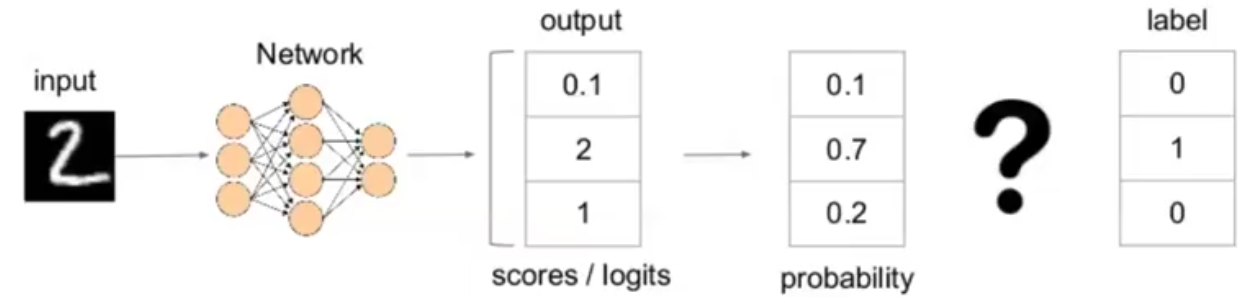
\includegraphics[width=.75\textwidth]{051}
    \caption{}
\end{figure}

\subsubsection{Activation function}
The activation functions are implemented inside the \textbf{hidden units}, because here we compute affine transformation \(z = W^Tx + b\), and the non-linearity is applied that we define as \(h(z)\). There are a lot of choices for \(h\), so we have to choose it wisely.

The design of the hidden units is an active area of research. However the most popular is the \textbf{ReLU}, where \(h(x) = \max(0,x)\). Here, the gradient is 0 or 1, similar to the linear units, easy to optimize. In fact it gives 1 if the gradient unit is active.

Potential problems with the ReLU activation function are that it is non-differentiable at zero, however, it is differentiable anywhere else, and the value of the derivate at zero can be arbitrarily chose to be 0 or 1; it is not zero-centered and it is unbounded; furthermore, the bigger problem is the \textbf{dying ReLU problem}: neurons can sometimes be pushed into states in which they become inactive for essentially all inputs. In this state, no gradients flow backward through the neuron, and so the neuron becomes stuck in a perpetually inactive state and \emph{dies}. This is a form of the vanishing gradient problem. In some cases, large numbers of neurons in a network can become stuck in dead states, effectively decreasing the model capacity. This problem typically arises when the learning rate is set too high. 

In order to mitigate these problems, there are some variants,for example: the Leaky ReLU, with \(y_i = a_ix_i\); the Randomized Leaky ReLU, with \(y_{ji} = a_{ji}x_{ji}\). 

Other variation of activation function are classical squashing type of non-linearity, for example the \textbf{Sigmoid}, with \(h(x) = \frac 1 {1 + e^{-x}}\) and the \textbf{Hyperbolic tangent}, with \(h(x) = \frac {e^x - e^{-x}} {e^x + e^{-x}}\).

\subsubsection{Architecture}
How do we decide the depth and the width of a neural network? There are not many theoretical advice for that, the only relevant result is that 2-layer net with linear output with some squashing non-linearity in hidden units can approximate any continuous function over compact domain to arbitrary accuracy (given enough hidden units).

The theorem also holds for other non-linear functions. The implication of this theorem is that regardless of function we are trying to learn, we know a large MLP can represent this function.

However, we are not guaranteed that our training algorithm will be able to learn that function.

\section{Backpropagation}
Backpropagationis a widely used algorithm for training feedforward neural networks. In fitting a neural network, backpropagation computes the gradient of the loss function with respect to the weights of the network for a signle input-output example, and does so efficiently, unlike a naive direct computation of the gradient with respect to each weight individually. This efficiency makes it feasible to use gradient methods for training multilayer networks, updating weights to minimize loss; gradient descent, or variants, are commonly used. The backpropagation algorithm works by computing the gradient of the loss function with respect to each weight by the chain rule, computing the gradient one layer at a time, iterating backward from the last layer to avoid redundant calculations of intermediate terms in the chain rule; this is an example of dynamic programming.

The idea of backpropagation is a flow starting from the input layers and goes on through the hidden layers until they reach the output layer. Then the computed prediction of the network is compared with the ground truth and the error signal is computed. The error signal is backpropagated to the network in order to compute the gradient and to update all the weights associated to this connection.

There are three main steps:
\begin{enumerate}
    \item \textbf{Feedforward propagation}: accept input \(x\), pass through intermediate stages and obtain output;
    \item Use the computed output to compute a \textbf{scalar cost} depending on the loss function;
    \item \textbf{Backpropagation} allows information to flow backwards from cost to compute the gradient.
\end{enumerate}

In backpropagation we use \textbf{gradient descent}: we need error derivatives for all the weights in the net.
\begin{equation}
    w^{(1)}_{11} := w^{(1)}_{11}-\eta \frac {\delta L} {\delta w^{(1)}_{11}}
\end{equation}
From the training data we do not know what the hidden units should do, but we can compute hwo fast the error changes as we change a hidden activity.

Each hidden unit can affect many output units and have separate effeccts on error, then we combine these effects. We can compute the \textbf{error derivatives for hidden units efficiently}. Once we have error derivatives for hidden activities, it is easy to get error derivatives for weights going in.

\subsection{Step 1: Feedforward propagation}
\begin{figure}[h]
    \centering
    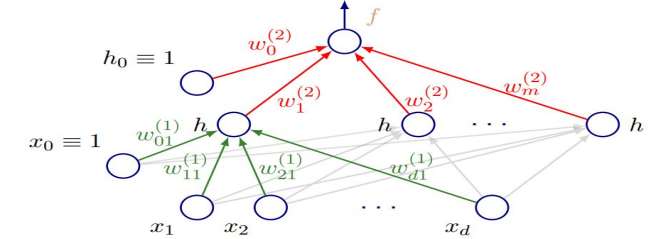
\includegraphics[width=.75\textwidth]{052}
    \caption{Feedforward operation.}
    \label{fig:052}
\end{figure}
In this step we go from our input to the output, with respect to Figure~\ref{fig:052}
\begin{equation}
    \hat{y} (\vec{x}; \vec{w}) = f \left( \sum_{j=1}^m w_j^{(2)} h \left( \sum_{i=1}^d w_{ij}^{(1)} x_i + w_{0j}^{(1)} \right) + w_0^{(2)} \right)
\end{equation}

\subsection{Step 2: Compute error and train}

The error of the network on a training set is
\begin{equation}
    L(X; \vec{w}) = \sum_{i=1}^N \frac 1 2 (y_i - \hat{y}(\vec{x}_i; \vec{w}))^2
\end{equation}
There is no closed-form solution. To train, we need to apply the gradient descent.

It means that we need to evaluate the derivative of \(L\) on a single example. We can consider a simple linear model for output \(\hat{y} = \sum_j w_j x{ij}\):
\begin{equation}
    \frac {\delta L(\vec{x}_i)} {\delta w_j} = (\hat{y}_i - y_i) x{ij}
\end{equation}

\subsection{Step 3: Backpropagation}
We need to compute the derivative of the error with respect to the weights, and these weights are the weights associated to the intermediate layers. The general unit activation in a multilayer network is
\begin{equation}
    z_t = h \left( \sum_j w_{jt} z_j \right)
\end{equation}

In forward propagation we calculate for each unit \(a_t = \sum_j w_{jt} z_j\). The loss \(L\) depends on \(w_{jt}\) only through \(a_t\). We are interested on computing
\begin{equation}
    \frac {\delta L} {\delta w_{jt}} = \frac{\delta L} {\delta a_t} \frac {\delta a_t} {\delta w_{jt}} = \frac {\delta L} {\delta a_t} z_j
\end{equation}
Now we are left of the problem of computing \(\frac {\delta L} {\delta a_t} z_j\). The key idea of backpropagation is that it can be computed recursively starting from the final layer to the earliest layer.

In the case of the last layer, \(\frac {\delta L} {\delta a_t} z_j\) corresponds to \(\hat{y} - y\), this is called the final error. The local error associated to the earlies layer can be computed as follows:
\begin{equation}
    \frac {\delta L} {\delta a_t} z_j = \sum_{s \in S} \frac {\delta L} {\delta a_s} \frac {\delta a_s} {\delta a_t} = h'(a_t) \sum_{s \in S} w_{ts} \frac {\delta L} {\delta a_s} z_j
\end{equation}
where \(a_s = \sum_{j:j \to s} w_{js} h(a_j)\).

\section{Training a Neural Network}
While training a Feedforward network, we need to do some modeling choices, for instance, we need to choose: the cost function, the form of output, the activation functions, the architecture (e.g. number of layers), and the \textbf{optimizer} (for the training).

Given a set of training samples \(T = \{(x_1, y_1), (x_2, y_2), ..., (x_N, y_N)\}\), the main idea of the training is to adjust all the weights of the network \(\Theta\) such that a cost function is minimized:
\begin{equation}
    \min_\Theta \sum_i L\left(y_i, f(x_i, \Theta)\right)
\end{equation}
We have to choose our loss function (e.g. L2, cross-entropy), and update the weights of each layer with gradient descent. It can be used the backpropagation of the error signal to compute the gradient efficiently.

\subsection{Gradient Descent}
Recall that the gradient is the vector of partial derivates with respect to all the coordinates of the weights:
\begin{equation}
    \nabla_wL = \left[ \frac {\delta L} {\delta w_1} \frac {\delta L} {\delta w_2} \cdots \frac {\delta L} {\delta w_N} \right]
\end{equation}
Each partial derivate measures how fast the loss changes in one direction. When the gradient is zero, i.e. all the partials derivates are zero, the loss is not changing in any direction.

Gradient descent finds the set of parameters that makes the loss as small as possible. The change of parameters depends on the gradients of the loss with respect to the network weights. Backpropagation is a method for computing gradient.

In order to define our optimization methods, let's see first the \textbf{Gradient Descent Rule}
\begin{algorithm}
    \caption{Vanilla Gradient Descent}
    \label{alg:vanilla_grad_desc}
\While{True}{
    $weights\_grad \gets $ evaluate\_gradient($loss\_fun$, $data$, $weights$)\;
    $weights \gets weights + step\_size \cdot weigths\_grad$\;
}
\end{algorithm}

\subsubsection{Batch Gradient Descent}
In BGD, all the training data is taken into consideration to take a single step. We take the average of the gradients of all the training example and then use that mean gradient to update our parameters. So that's just one step of gradient descent in one epoch.

\begin{algorithm}
    \caption{BatchGradientDescent($k$)}
    \label{alg:batch_gradient_descent}
\KwData{Learning rate $\epsilon_k$}
\KwData{Initial parameter $\Theta$}
    \While{stopping criteria is not met}{
        Compute gradient estimate over $N$ examples:\\
        $\hat{g} \gets \frac 1 N \nabla_\Theta \sum_i L\left( f(\vec{x}^{(i)}; \Theta), \vec{y}^{(i)} \right)$\;
        Apply Update: $\Theta \gets \Theta - \epsilon \hat{g}$\;
    }
\end{algorithm}

A pro of this algorithms is that the gradient estimates are stable, on the other hand it need to compute gradients over the entire training for one update.

\subsubsection{Stochastic Gradient Descent}
To tackle this problem we have Stochastic Gradient Descent. In Stochastic Gradient Descent (SGD), we consider just one example at a time to take a single step.

\begin{algorithm}
    \caption{StochasticGradientDescent($k$)}
    \label{alg:stochastic_gradient_descent}
\KwData{Learning rate $\epsilon_k$}
\KwData{Initial parameter $\Theta$}

    \While{stopping criteria is not met}{
        Sample example $(\vec{x}^{(i)}, \vec{y}^{(i)})$ from training set\;
        Compute gradient estimate:\\
        $\hat{g} \gets \nabla_\Theta L\left( f(\vec{x}^{(i)}; \Theta), \vec{y}^{(i)} \right)$\;
        Apply Update: $\Theta \gets \Theta - \epsilon \hat{g}$\;
    }
    
\end{algorithm}

A problem with this algorithm is that gradient estimates can be very noisy. One possible solution can be to use larger \textbf{mini-batches}. The advantage is that the computation time per update does not depend on the number of training examples \(N\), so it permits computation on extremely large datasets. This solution is often done with a parallel implemenetation. Using GPUs it is common for power of 2 batch sizes to offer better runtime (some kinds of hardware achieve better runtime with specific sizes of arrays).

\subsubsection{Momentum}
The progress to the minimum with SGD is very slow along a flat direction, it causes jitter along the steep one.

So we can use the SDG with \textbf{momentum}, that introduces a new variable \(\vec{v}\), the velocity. The velocity is an exponentially decaying moving average of the negative gradient.

\begin{algorithm}
    \caption{StochasticGradientDescent with Momentum}
    \label{alg:stochastic_gradient_descent_momentum}
\KwData{Learning rate $\epsilon_k$}
\KwData{Momentum parameter $\alpha$}
\KwData{Initial parameter $\Theta$}
\KwData{Learning velocity $\vec{v}$}

    \While{stopping criteria is not met}{
        Sample example $(\vec{x}^{(i)}, \vec{y}^{(i)})$ from training set\;
        Compute gradient estimate:\\
        $\hat{g} \gets \nabla_\Theta L\left( f(\vec{x}^{(i)}; \Theta), \vec{y}^{(i)} \right)$\;
        Compute the velocity update:\\
        $\vec{v} \gets \alpha \vec{v} - \epsilon \hat{g}$\;
        Apply Update: $\Theta \gets \Theta - \vec v$;
    }
    
\end{algorithm}

\subsubsection{Adaptive Learning Rate Methods}
So far we have assigned the same learning rate to all features. If the features vary in importance and frequency, is this a good idea? The learning rate is one of the hyperparameters most difficult to set.

\section{Convolutional Neural Networks}
\textbf{Convolutional Neural Network} (CNN or ConvNet) is a class of artificial neural network, most commonly applied to analyze visual imagery.  Neural networks are extremely powerful in applications that deal with an input space which is locally structured, i.e. spatial or temporal, for example images and language, and that deal with an arbitrary input of features.

The name "convolutional neural network" indicates that the network employs a mathematical operation called convolution. Convolutional networks are a specialized type of neural networks that use convolution in place of general matrix multiplication in at least one of their layers.

A convolutional neural network consists of an input layer, hidden layers and an output layer. In any feed-forward neural network, any middle layers are called hidden because their inputs and outputs are masked by the activation function and final convolution. In a convolutional neural network, the hidden layers include layers that perform convolutions.

\subsection{Convolutional layers}
In a CNN, the input is a tensor with a shape: given the number of inputs \(n\), the input height \(h\), the input width \(w\), and the input channels \(c\), the shape \(s\) is defined as:
\begin{equation}
    s = n \cdot h \cdot w \cdot c
\end{equation}
After passing through a conolutional layer, the image becomes abstracted to a feature map, also called an activation map.

Convolutional layers convolve the input and pass its result to the next layer. This is similar to the response of a neuron in the visual cortex to a specific stimulus. Each convolutional neuron processes data only for its receptive field. Although fully connected feedforward neural network can be used to learn features and classify data, this architecture is generally impractical for larger inputs such as high resolution images. It would require a very high number of neurons, even in a shallow architecture, due to the large input size of images, where each pixel is a relevant input feature. For instance, a fully connected layer for a (small) image of size 100 x 100 has 10,000 weights for each neuron in the second layer. Instead, convolution reduces the number of free parameters, allowing the network to be deeper. For example, regardless of image size, using a 5 x 5 tiling region, each with the same shared weights, requires only 25 learnable parameters. Using regularized weights over fewer parameters avoids the vanishing gradients and exploding gradients problems seen during backpropagation in traditional neural networks.

In practice, CNN learns a hierarchy of features. Each layer of hierarchy extracts features from the output of the previous layer, and then trains all layers jointly.

Furthermore, convolutional neural networks are ideal for data with a grid-like topology (such as images) as spatial relations between separate features are taken into account during convolution and/or pooling.

\begin{figure}[h!]
    \centering
    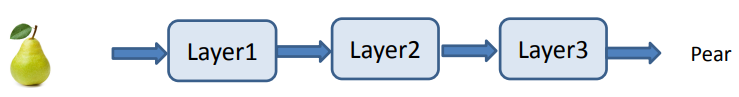
\includegraphics[width=.75\textwidth]{055}
    \caption{}
    \label{fig:055}
\end{figure}

Convolutional neural networks are Feedforward neural networks with a specialized connectivity structure, where multiple layers of feature extractors are stacked: low-level layers extract local features, and high-level layers learn global patterns. Typically CNN layers transform the input matrix into an output class prediction. There are a few distinct types of operations:
\begin{itemize}[topsep={0pt}, partopsep={0pt}]
    \itemsep0pt
    \item Convolution
    \item Non-linearity
    \item Pooling
\end{itemize}

\subsubsection{Convolution}
\begin{wrapfigure}{l}{0.35\textwidth}
    \begin{center}
        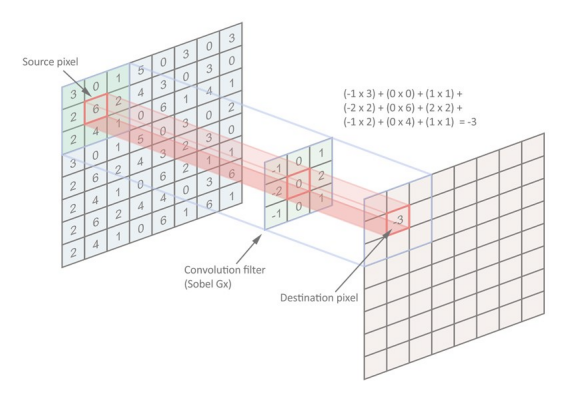
\includegraphics[width=0.25\textwidth]{056}
        \caption{}
    \end{center}
    \label{fig:056}
\end{wrapfigure}

The convolution is a mathematical operation on two functions \(f\) and \(g\) that produces a third function \(f \cdot g\) that expresses how the shape of one is modified by the other. It is a general purpose filter operation for images. A kernel matrix is applied to an image, and it works by determining the value of a central pixel by adding the weighted values of all its neighbors together. The output is a new modified (filtered) image, and it can be used to smooth, sharpen, enhance, etc.
\begin{equation}
    S(i,j) = (I \cdot K)(i,j) = \sum_m \sum_n I(m,n)K(i-m,j-n)
\end{equation}

The convolution layer is the core layer of the CNN, it consists of a set of filters, and each filter covers a spatially small portion of the input data (receptive field) and is convolved across the dimensions of the input data, producing a multi-dimensional feature map.

\begin{wrapfigure}{r}{0.35\textwidth}
    \begin{center}
        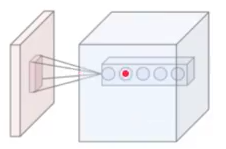
\includegraphics[width=0.25\textwidth]{058}
        \caption{}
    \end{center}
    \label{fig:058}
\end{wrapfigure}

The intuition is that the network will learn filters that activate when they see some specific type of feature at some spatial position in the input.

The filter is smaller than the input data and the type of multiplication applied between a filter-sized patch of the input and the filter is a dot product. A dot product is the element-wise multiplication between the filter-sized patch of the input and filter, which is then summed, always resulting in a single value. Because it results in a single value, the operation is often referred to as the “scalar product“.

Using a filter smaller than the input is intentional as it allows the same filter (set of weights) to be multiplied by the input array multiple times at different points on the input. Specifically, the filter is applied systematically to each overlapping part or filter-sized patch of the input data, left to right, top to bottom.

\begin{figure}[h!]
    \centering
    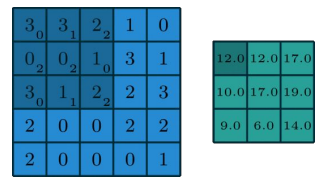
\includegraphics[width=.5\textwidth]{057}
    \caption{An example of an input data with a filter and the output of the total convolution.}
    \label{fig:057}
\end{figure}

\subsubsection{Non-linearity}
After the convolution, the non-linearity is computed. The result of the convolution as in the feedforward neural network is then passwd to an activation function (e.g. ReLO or Sigmoid)
\begin{align*}
    y_{i,j} = &f(a_{i,j})\\
    \text{e.g. } &f(a) = \left[a\right]_+\\
    &f(a) = sigmoid(a)
\end{align*} 
We are using non-linearity in order to have a final non-linear representation for our prediction model and, more importantly, since the non-linearity is applied element-wise, it does not affect the receptive field of the neural network.

\subsubsection{Spatial Pooling}
After the application of the non-linearity, there is a downsampling operation, called \textbf{spatial pooling}, and it is used to provide invariance to small traslation of the input.

There are several non-linear functions to implement pooling, where max pooling is the most common. It partitions the input image into a set of rectangles and, for each such sub-region, outputs the maximum. 

Intuitively, the exact location of a feature is less important than its rough location relative to other features. This is the idea behind the use of pooling in convolutional neural networks. The pooling layer serves to progressively reduce the spatial size of the representation, to reduce the number of parameters, memory footprint and amount of computation in the network, and hence to also control overfitting. This is known as down-sampling. It is common to periodically insert a pooling layer between successive convolutional layers (each one typically followed by an activation function, such as a ReLU layer) in a CNN architecture.
\begin{equation}
    x_{i,j} = \max_{|k| < \tau , |l| < \tau} y_{i-k,j-l}
\end{equation}

\begin{figure}[h!]
    \centering
    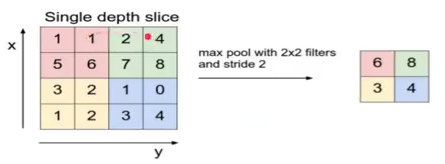
\includegraphics[width=.75\textwidth]{059}
    \caption{Example of max pooling.}
    \label{fig:059}
\end{figure}

\section{Other Neural Networks}
\begin{figure}[t!]
    \centering
    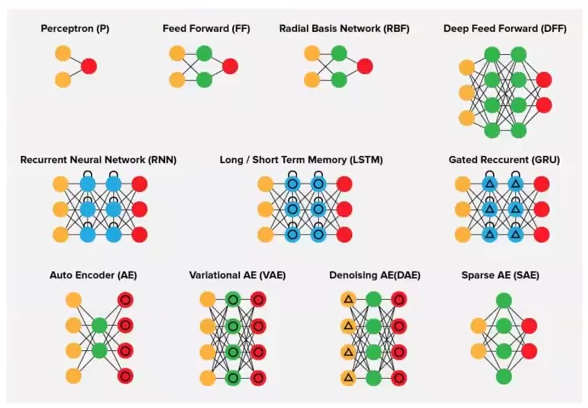
\includegraphics[width=.75\textwidth]{060}
    \caption{Many models for different needs.}
    \label{fig:060}
\end{figure}

In particular so far we have discussed the Perceptron, the Feedforward neural network, and the Deep Feedforward neural network, where we have multiple hidden layers.

So far, we focused mainly on prediction problems with fixed-size inputs and outputs. We discussed the flexibility of CNN to address a wide range of task, but what if the input and/or output is a variable-length sequence? There are many applications where we need this, for example document classification, sentiment analysis, or image captioning.

\subsection{Recurrent Neural Networks}
For this problem, different type of neural networks are required. Let's consider an example, a video frame prediction, given a video, the model should predict the category of each frame of the video --- this example could be useful for segmenting a movie in different parts. Until now, we have seen a \textbf{Single2Single} type of neural network, the feedforward neural network, where we have given a single object as input and we want to predict a single object as output. But for this problem we need to implement a \textbf{Multiple2Multiple} network, the \textbf{Recurrent Network}, that has been designed in problems in which we have multiple object as input and we want to predict multiple objects as output. Note that there is another type of neural network, the \textbf{Single2Multiple}, where I have for example a single image and I want to predict multiple captions of the image.

For the problems above, Feedforward neural networks and Convolutional neural networks cannot be applied. The choice in this case is to apply another type of neural network, where, given an input \(x_t\), the neural network passes the input to an input layer that learns an hidden representation \(h_t\) that could be eventually used by a classifier to perform some output prediction \(y_t\).

Notice that the particularity of the Recurrent Neural Network is the \textbf{recurrence formula}, that is a function of certain parameters of the network that relates the input at time \(t\) and the latent representation of the previous state with the latent representation of the current state:
\begin{equation}
    h_t = f_W(x_t, h_{t-1})
\end{equation}
These recurrents operations take into account the concept of time/sequence processing, and can be better understood by unrolling the formula with the scheme in Figure~\ref{fig:061}. 
\begin{figure}[h!]
    \centering
    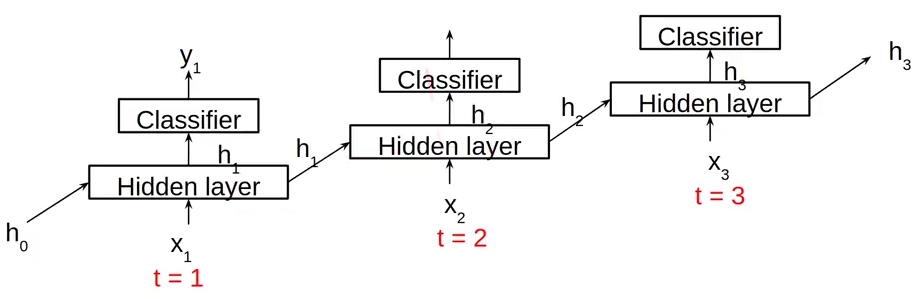
\includegraphics[width=.75\textwidth]{061}
    \caption{Recurrent neural network.}
    \label{fig:061}
\end{figure}

\subsection{Autoencoders}
\textbf{Autoencoders (AE)} are somwhat similar to FFNNs as AEs are more like a different use of FFNNs than a fundamentally different architecture. The basic idea behind autoencoders is to encode information (as in compress, not encrypt) automatically, hence the name. The entire network always resembles an hourglass like shape, with smaller hidden layers than the input and output layers. AEs are also always symmetrica around the middle layer(s). The smalles layers are almost always in the middle, the place where the information is most compressed. Everything up to the middle is called the encoding part, everything after the middle the deconding and the middle is called the code. One can train them using backpropagation by feeding input and setting the error to be the difference between the input and what came out. AEs can be built symmetrically when it comes to weights as well, so the encoding weights are the same as the decoding weights.

Autoencoders can be considered as an unsupervised approach for learning a lower-dimensional feature representtion from unlabeled data.

\begin{figure}[h!]
    \centering
    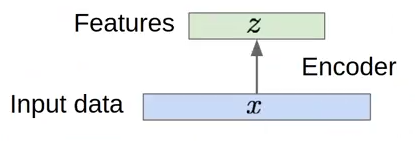
\includegraphics[width=.5\textwidth]{062}
    \caption{Autoencoders scheme example.}
    \label{fig:062}
\end{figure}

For instance, if the input is a bunch of image, in the autoencoder there is a network --- the encoder network --- that maps the original input data into low-dimensional latent representations.

Encoders can be realized in several ways, for instance they can be realized by linear layers + nonlinearity (e.g. sigmoid), can be realized by a deep fashion by concatenating multiple fully-connected layers, or it can be realized in a convolutional fashion by having some convolutional layers and ReLU activation function one after the other.

\begin{wrapfigure}{l}{0.35\textwidth}
    \begin{center}
        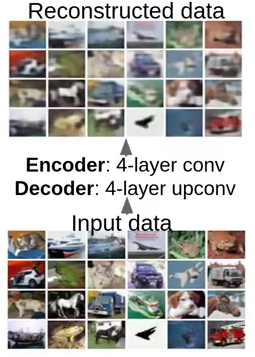
\includegraphics[width=0.25\textwidth]{064}
        \caption{}
    \end{center}
    \label{fig:064}
\end{wrapfigure}

Independently of the encoder, the main idea is that the representation of the output \(z\) should be smaller than the input \(x\), so the encoder should perform dimensionality reduction. 

How to learn this feature representation? The idea is to train the autoencoder so that features can be used to reconstruct original data --- autoencoding: encoding itself.

Once we decided the architecture of the encoder and the consequent architecture of the decoder, we need a loss function, and in the case of the autoencoders the loss function is a reconstruction function that minimizes the difference between the original data and the reconstructed version of the input data:
\begin{equation}
    ||x - \hat{x}||^2
\end{equation}
\begin{figure}[h!]
    \centering
    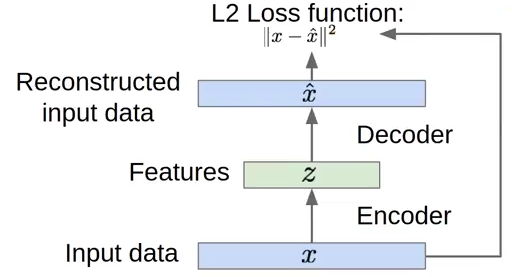
\includegraphics[width=.5\textwidth]{063}
    \caption{Autoencoders with loss function.}
    \label{fig:063}
\end{figure}

Autoencoders are aimed to learn the latent representation \(z\), so the most common use of autoencoders is to use the common feature \(z\) in order to initialize a feature model. This means that once we have trained the autoencoder, we throw away the decoder, and we only take the latent representation \(z\) and we append the loss funcion \(\hat{y}\) and the the encoder now can be used to have a better initialization of a supervised model.

\newpage
\begin{exercise}[topsep=20pt,itemsep=10pt]
    \ex Describe a general neural network.
    \ex[!] Describe the Feedforward Neural Networks.
    \ex[!] What is backpropagation? Describe it's steps.
    \ex How do we train a neural network?
    \ex Describe the Batch Gradient Descent.
    \ex Describe the Stohastic Gradient Descent.
    \ex[!] What is the momentum? How do we update the neural network with the momentum?
    \ex Describe the momentum paramether \(\alpha\), how does it influence the momentum?
    \ex[!] Describe the Convolutional Neural Networks.
    \ex[!] Describe the Convolution layer.
    \ex[!] What is the non-linearity in the neural network? Where do we apply it?
    \ex[!] Describe the Spatial Pooling.
    \ex[!] What is a Recurrent Neural Network? For what kind of tasks do we use it?
    \ex[!] Describe the Autoencoders.
    \ex[!] What is ResNet?
\end{exercise}